\section*{Q4 [30 Marks]}

Consider a simple neural network with a single hidden layer. 
The input layer consists of three-dimensional \( \mathbf{x} = (x_1, x_2, x_3)^T \). 
The hidden layer includes two-dimensional \( \mathbf{h} = (h_1, h_2) \). 
The output layer includes one scalar \( o \). 
We ignore bias terms for simplicity.

We use linear rectified (ReLU) as activation function \textbf{for the hidden and output layer BOTH}.
\begin{equation*}
    \text{ReLU}(x) = \max(0, x)
\end{equation*}
\begin{equation*}
    \text{ReLU}'(x) = 
        \begin{cases} 
        1, & \text{if } x > 0 \\
        0, & \text{if } x \leq 0 
        \end{cases}
\end{equation*}

Moreover, denote the loss function (also called error in slides) by \( \mathbf{J}(o, t) = \frac{1}{2} |o - t|^2 \).
where \( t \) is the associated label (target) value for scalar output \( o \).
Denote by \( W \) and \( V \) weight matrices connecting input and hidden layer, and hidden layer and output respectively.
They are \textbf{initialized} (i.e., the initial condition before the first updating round) as follows:
\begin{equation}
W = \begin{bmatrix}
1 & 0 & 1 \\
-3 & -1 & 0 \\
\end{bmatrix}, 
V = \begin{bmatrix}
0 & 1
\end{bmatrix},
\end{equation}

Now, try to solve the following parts.

\begin{itemize}
    \item[(a)] (5 marks) Write out symbolically (thus, no need to plug in the specific values of \( W \) and \( V \) just yet) the mapping \( \mathbf{x} \rightarrow o \) using ReLU, \( W \), \( V \).
    \item[(b)] (10 marks) Given the condition \( \mathbf{x} = (1, 2, 1)^T, t = 1 \), compute the numerical output value \( o \), clearly show all intermediate steps. You can reuse the results of the previous question.
    \item[(c)] (15 marks) Compute the gradient of the loss function with respect to the \( V \) weights, and evaluate the gradients at specific \( \mathbf{x} = (1, 2, 1)^T, t = 1 \).
\end{itemize}

\subsection*{Solution:}

\paragraph*{(a)}

\begin{center}
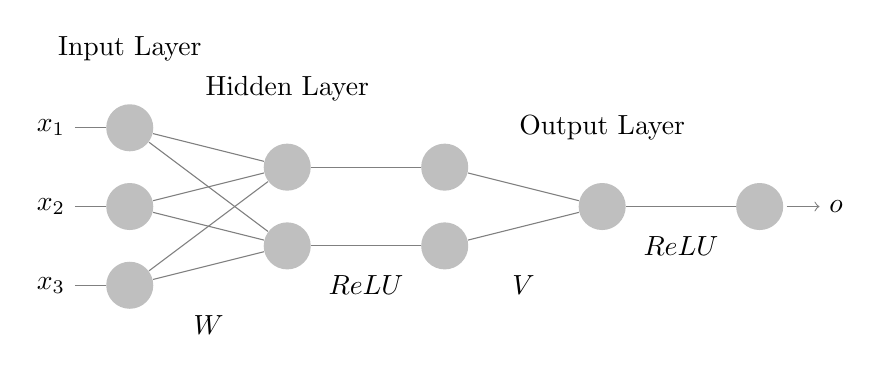
\begin{tikzpicture}[-,draw=black!50, node distance=2cm]
    \tikzstyle{every pin edge}=[<-,shorten <=1pt]
    \tikzstyle{neuron}=[circle,fill=black!25,minimum size=17pt,inner sep=0pt]

    % Input value
    \node at (-1,-1) (x1) {$x_1$};
    \node at (-1,-2) (x2) {$x_2$};
    \node at (-1,-3) (x3) {$x_3$};

    % Input layer
    \foreach \y in {1,2,3}
        \node[neuron] (I-\y) at (0,-\y) {};

    % Hidden layer
    \foreach \y in {1,2}
        \node[neuron] (H-\y) at (2,-\y-0.5) {};

    % Activation layer of hidden layer
    \foreach \y in {1,2}
        \node[neuron] (Ah-\y) at (4,-\y-0.5) {};

    % Output layer
    \node[neuron] (O) at (6,-2) {};

    % Activation layer of output layer
    \node[neuron,pin={[pin edge={->}]right:$o$}] (Ao) at (8,-2) {};

    % Connect input value to input layer
    \draw (x1) -- (I-1);
    \draw (x2) -- (I-2);
    \draw (x3) -- (I-3);

    % Connect input to hidden
    \foreach \src in {1,2,3}
        \foreach \dst in {1,2}
            \draw (I-\src) -- (H-\dst);

    % Connect hidden to activation
        \draw (H-1) -- (Ah-1);
        \draw (H-2) -- (Ah-2);

    % Connect activation of hidden to output
    \foreach \src in {1,2}
        \draw (Ah-\src) -- (O);

    % Connect activation of output to activation
    \draw (O) -- (Ao);
        
    % Annotate layers
    \node[above of=I-1, node distance=1cm] (l1) {Input Layer};
    \node at (1,-3.5) (l2) {$W$};
    \node[above of=H-1, node distance=1cm] (l3) {Hidden Layer};
    \node at (3,-3) (l4) {$ReLU$};
    \node at (5,-3) (l5) {$V$};
    \node[above of=O, node distance=1cm] (l6) {Output Layer};
    \node at (7,-2.5) (l7) {$ReLU$};

\end{tikzpicture}
\end{center}

\paragraph*{(b)}

The output of the hidden layer can be computed as \( \mathbf{h} = \text{ReLU}(W \cdot \mathbf{x}) \).
    \[
    \mathbf{h} = \text{ReLU}\left(\begin{pmatrix} 1 & 0 & 1 \\ -3 & -1 & 0 \end{pmatrix} \begin{pmatrix} 1 \\ 2 \\ 1 \end{pmatrix}\right)
    = \text{ReLU}\left(\begin{pmatrix} 2 \\ -5 \end{pmatrix}\right)
    = \begin{pmatrix} 2 \\ 0 \end{pmatrix}
    \]

The output \( o \) can be computed as \( o = \text{ReLU}(V \cdot \mathbf{h}) \).  
    \[
    o = \text{ReLU}\left(\begin{pmatrix} 0 & 1 \end{pmatrix} \begin{pmatrix} 2 \\ 0 \end{pmatrix}\right)
    = \text{ReLU}(0)
    = 0
    \]

So, the numerical output value \( o \) would be 0 given the condition \( \mathbf{x} = (1, 2, 1)^T \) and \( t = 1 \).

\paragraph*{(c)}

Because the given loss function is 
\[
J(o, t) = \frac{1}{2} |o - t|^2
\]
where \( o \) is the predicted output and \( t \) is the target value.

Then we have:
\[
\frac{\partial J}{\partial o} = o - t
\]

Since \( o = \text{ReLU}(V \cdot h) \), and \( h = (2, 0)^T \) (from earlier calculation), \( \frac{\partial o}{\partial V} = h \) if \( o > 0 \) and \( \frac{\partial o}{\partial V} = 0 \) otherwise.

Finally, use the chain rule to find \( \frac{\partial J}{\partial V} \):
\[
\frac{\partial J}{\partial V} = \frac{\partial J}{\partial o} \times \frac{\partial o}{\partial V}
\]

Evaluate the Gradients:

\begin{itemize}
    \item[1.] \( \frac{\partial J}{\partial o} = o - t = 0 - 1 = -1 \)
    \item[2.] \( \frac{\partial o}{\partial V} = 0 \) (because \( o = 0 \) which is not greater than 0)
    \item[3.] \( \frac{\partial J}{\partial V} = -1 \times 0 = 0 \)
\end{itemize}

So, the gradient of the loss function with respect to the \( V \) weights is 0.
